% Likert Scale

\documentclass[tikz = true, border = 2pt]{standalone}
\usepackage{amsmath}
\usepackage{amsfonts}
\usepackage{amssymb}
\usepackage{graphicx}
\usepackage{tikz}
\usetikzlibrary{positioning, calc}
\usetikzlibrary{intersections}
\usetikzlibrary{decorations.pathreplacing}
\usetikzlibrary{decorations.text}
\usetikzlibrary{arrows,shapes,backgrounds, shadows,fadings}
\usepackage{fontspec}
\setmainfont{Equity Text A}[SmallCapsFont={Equity Caps A}]
\begin{document}
	
	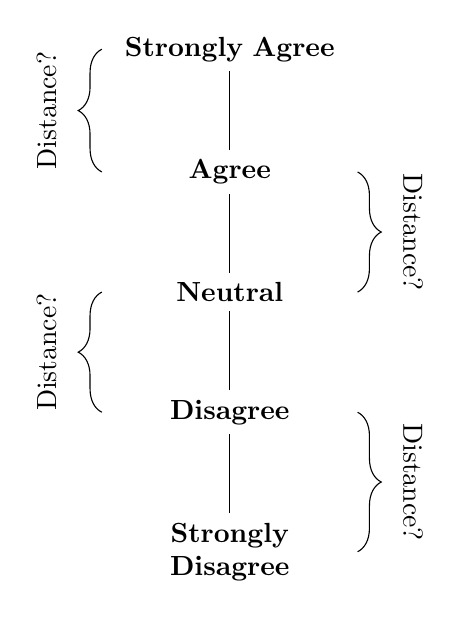
\begin{tikzpicture} [font=\normalsize]
	\node [align=center,text width=3cm] (sd)  {\textbf{Strongly Disagree}};
	\node [align=center,text width=3cm,above=of sd]  (d) {\textbf{Disagree}};
	\node [align=center,text width=3cm,above=of d]  (n) {\textbf{Neutral}}; 
	\node [align=center,text width=3cm,above=of n] (a)  {\textbf{Agree}};
	\node [align=center,text width=3cm,above=of a] (sa) {\textbf{Strongly Agree}};
	\draw [decoration={brace,amplitude=3mm}, decorate] (d.east) -- (sd.east) node[midway, rotate=-90,align=center,yshift=2em]{Distance?};
	\draw [decoration={brace,amplitude=3mm}, decorate] (d.west) -- (n.west) node[midway, rotate=90,align=center,yshift=2em]{Distance?};
	\draw [decoration={brace,amplitude=3mm}, decorate] (a.east) -- (n.east) node[midway, rotate=-90,align=center,yshift=2em]{Distance?};
	\draw [decoration={brace,amplitude=3mm}, decorate] (a.west) -- (sa.west) node[midway, rotate=90,align=center,yshift=2em]{Distance?};
	\draw (sd.north) -- (d.south);
	\draw (d.north) -- (n.south);
	\draw (n.north) -- (a.south);
	\draw (a.north) -- (sa.south);
	\end{tikzpicture}
\end{document}